\documentclass[11pt,a4paper]{article}
\usepackage[utf8]{inputenc}
\usepackage{amsmath}
\usepackage{amsfonts}
\usepackage{amssymb}
\usepackage{listings}
\usepackage{graphicx}
\usepackage{listings}
\usepackage{babel}[german]
% for pseudocode
\usepackage{algorithm}
\usepackage[noend]{algpseudocode}

% for code style
\usepackage{xcolor}

\definecolor{codegreen}{rgb}{0,0.6,0}
\definecolor{codegray}{rgb}{0.5,0.5,0.5}
\definecolor{codepurple}{rgb}{0.58,0,0.82}
\definecolor{backcolour}{rgb}{0.95,0.95,0.92}

\lstdefinestyle{mystyle}{
    backgroundcolor=\color{backcolour},   
    commentstyle=\color{codegreen},
    keywordstyle=\color{magenta},
    numberstyle=\tiny\color{codegray},
    stringstyle=\color{codepurple},
    basicstyle=\ttfamily\footnotesize,
    breakatwhitespace=false,         
    breaklines=true,                 
    captionpos=b,                    
    keepspaces=true,                 
    numbers=left,                    
    numbersep=5pt,                  
    showspaces=false,                
    showstringspaces=false,
    showtabs=false,                  
    tabsize=2
}

\lstset{style=mystyle}
% ----------------------

% usesul macros
\newcommand{\lstin}[1]{\lstinline[language=C]{#1}}

\author{Christoph Pooch}
\title{\underline{Hashmap - eine Implementierung in C}}
\begin{document}
\maketitle
\pagebreak
\tableofcontents
\pagebreak
\section{Einleitung}
Diese Arbeit befasst sich mit der Umsetzung des Konzeptes einer Hashmap in der Programmiersprach C.
Eine Hashmap, wie in einem Folgenden Abschnitt noch näher erläutert, stellt einen Kompromiss zwischen 
Speichernutzung und Zugriffszeit da.
Hierfür wird ein Datensatz (Value) auf einen Schlüssel (Key) abgebildet.
Nativ ist diese Datenstruktur in C nicht implementiert, was den Antrieb für diese Arbeit darstellt.
Nachdem das Prinzip und Konzept einer Hashmap erörtert wurden, wird in dieser Arbeit genau auf die Umsetzung 
eben dieser Datenstruktur als Bibliothek für die Programmiersprache C eingegangen und alle Funktionalitäten, 
wie auch Herangehensweisen erklärt.\\
Da es verschiedene Möglichkeiten der Umsetzung für Hashmaps gibt und es vorallem bei der Auswahl, noch 
später erläuterten, Hashfunktion eine große Vielzahl an Optinen gibt, die sich in ihrer Komplexität teilweise 
sehr unterschieden, habe ich mich auf eine relativ einfache Funktion festgelgt. %Fix me
In dieser ARbeit geht es immerhin um die Umsetzung der Funktionsweise einer Hashmap und nicht um die Implementierung 
einer komplexen Hashfunktion.\\\\ 
Für die Umsetzung dieses Projekts, der Implementierung einer Hashmap als Datenstruktur in C, wurden vorallem vier
Komponenten benutzt.\\
Ein Linuxsubsystem unter Windows-Subsystem für Linux (WSL/WSL2),
genauer Ubuntu 20.04. Dies diente der einfachen Nutzung der Programmiersprache C und des zugehörigen Compielers GCC, 
dies ist die zweite Komponente der Toolchain.\\
Als Entwicklungsumbegbung wurde Visual Studio Code (VSCode) verwendet, da dieses eine einfache Verknüpfung zur 
Ubuntu-Konsole bietet und man zusätzlich auch LaTeX und vieles mehr über die Extensionfunktion integrieren kann.
Letzteres wurde zum Schreiben dieser Arbeit verwendet.

\section{Konzept Hashmap}
\subsection{Assoziativer Speicher}

Eine Hashmap stellt konzeptuell eine Form von assoziativem Speicher dar.
Hierbei handelt es sich um eine Alternative zum Speicherzugriff über eine Speicheradresse.\\
Die Speicheradresse verweist üblicherweise auf Daten die an einer genau
beschriebenen Stelle im Speicher liegen. So werden auch in der, in dieser Arbeit verwendeten, Programmiersprache C Variablen
behandelt. Zu jeder Variable, unabhängig von ihrem Typ, gibt es eine Speicheradresse (Pointer), der auf die Stelle im Speicher
verweist, an der die Daten hinterlegt sind.\\
Alternativ funktioniert ein assoziativer Speicherzugriff über einen Speicherwert oder Schlüssel (Key). Dieser Schlüssel wird 
dann auf einen Datensatz abgebildet. Die Assoziation wird je nach Anwendungsfall anders geregelt. Bei Hashmaps wird das über 
eine Hashfunktion gelöst, welche den Schlüssel auf die Daten (Values) abbildet.\\
Man kann sich also eine Hashmap als eine Art Liste vorstellen, bei der zu einem Listenelement immer ein Key und ein Value gehören.
Diese sind eindeutig zugeordnet und so kann man schnell über die Eingabe eines Schlüssel-
wertes auf die gewünschten Daten zugreifen.
Dieser Ansatz eines assoziativen Speichers ist als Kopmromiss zwischen Zugriffszeit und Speichernutzung zu verstehen.
Hätte man unbegrenzte Zeit für die Suche nach dem ge- 
wünschten Wert in der Liste der Values, dann könnte man auf die Keys verzichten.
Man würde ganz einfach alle Listenelement nach und nach durchgehen, lesen und entscheiden ob es der Wert ist, nach dem man gesucht hat.
Das mag für kleinere Mengen von Werten gehen, wie etwa wenn man ein Buch in einem einzigen Regal sucht. Die Menge an Büchern ist limitiert
und somit auch die Zeit, die man für die Suche benötigt. Anders sähe das aus, wenn man das selbe Buch in einer ungeordneten Bibliothek sucht.
Es würde einen im Durchschnitt eine ganze Weile beschäftigen nach diesem speziellen Exemplar zu stöbern.\\
Hier kommen die Keys ins Spiel. Sie sorgen, wie bereits erwähnt, für eine eindeutige Zuordnung zwischen sich selbst und den Daten.
So hätte, in diesem Beispiel, jedes Buch eine Nummer über die man es direkt in einem Verzeichnis finden kann.
Doch es gibt auch hier ein Problem. Hat man eine sehr große Zahl von Einträgen in der Liste, dann benötigt man sehr lange, speicherintensive 
Schlüsselwerte, um die Eindeutigkeit zu gewährleisten. Man würde also zugunsten der Zugriffszeit den Speicher völlig ausfüllen.
Das kann nicht die Lösung sein und deshalb gibt es eine Limitierung für die Größe der Schlüsselwerte. Das wird über die Abbildung des Schlüssels 
auf einen Hashwert (Hash) bewerkstelligt.
Da man die Eindeutigkeit der Hashes nicht einhundertprozentig gewährleisten kann, handelt es sich um einen Kompromiss zwischen Zugriffszeit und Speichernutzung.\\

\subsection{Hashfunktion}

Im vorherigen Abschnitt wurde die Zuordnung von Keys zu ihren Values behandelt und es ist klar geworden, dass die Keys nicht unendlich groß sein können.
Um dieses Problem in den Griff zu bekommen, bildet man die Schlüsselwerte über eine Hashfunktion auf einen Hash ab.
Dieser Wert hat eine wesentlich kleinere Größe als der Schlüssel und man spart somit viel Speicherplatz.\\
Die drei wichtigsten Eigenschaften einer Hashfunktion sind die Eindeutigkeit der Abbildung von den Schlüsselwerten zu den Hashwerten, die Schnelligkeit 
der Ausführung dieser Abbildung und die Unumkehrbarkeit dieser Abbildung.\\
Vorallem die erste Eigenschaft, die Eindeutigkeit, hat eine besonders nützliche Auswirkung auf die Nutzung einer Hashmap. Da Keys und Hashes eindeutig zugeordnet sind,
beträgt die Suchkomplexität in einer optimalen Hashmap $O(1)$. Das stellt einen bedeutenden Vorteil gegenüber anderen Datenstrukturen dar. Beispielsweise hat eine 
verkettete Liste (LinkedList), deren Elemente hintereinander gespeichert, und über Pointer miteinander verbunden sind, eine Suchkomplexität von $O(n)$, wobei $n$ die Anzahl der Listenelemente ist.\\
Da allerdings der der Speicherbedarf in der Umsetzung eienr Hashmap ebenfalls eine Rolle spielt, wird - wie bereits erwähnt - gefordert, dass die Hashfunktion einen Hash 
ausgibt, dessen Speicherbedarf geriner ist, als der des Keys. Dass unter dieser Verkleinerung des Speicherbedarfs die Eindeutigkeit der Zuordnung leidet, lässt sich 
mit einem mathematischen Grundsatz, dem sogenannten Auswahlaxiom, begründen. Hat man eine größere Menge X an Elementen und versucht diese auf eine kleinere Menge Y abzubilden, so muss immer
mindestens ein Element der Menge X übrig bleiben, welches keine eindeutige Abbildung zu einem Gegenstück in der Menge Y erhält.
Man Spricht hierbei von einer Kollision.\\
Kollisionen sind bei einer Hashfunktion, neben der Dauer ihrer Ausfrührung, der ausschlaggebende Faktor. Verursacht eine Haashfunktion viele Kollisionen,
so ist sie nicht effizient. Ein Beispiel für eine solche Funktion, welche sehr einfach und schnell ausführbar ist, ist die Modulo-Operation.
Sie birgt als Hashfunktion den großen Nachteil vieler Kollisionen. Für eine Hashmap der Größe G und einem Key K als Eingabewert könnte eine Umsetzung folgendermaßen aussehen:
$$Hash = K~ mod ~G$$
Es ist offenkundig, dass bei der Nutzung der Modulo-Operation als Hashfunktion sehr viele Kollisionen auftreten werden. Jedoch lässt sich so sehr einfach das Prinzip
der Zuordnung von Keys und Values erklären, wie auch das Kollisionsproblem.
Zum Beispiel man eine Hashmap der Größe $G = 8$ an. Das bedeutet, das es acht mögliche Listenelement gibt, in die Werte geschriebe werden können.
In der Liste sollen Städtenamen gespeichert werden, dies sind die Values. Als Keys werden der Einfachheit halber beliebige Nummern gewählt, welche eindeutig sein sollen.
Die Hashfunktion bleibt die Modulo-Operation, wie oben abgebildet.\\
Zuerst wird die Stadt \textit{Berlin} mit dem Key $K = 1$ in die Hashmap eingefügt. Der Eintrag erfolgt an der Stelle $1~ mod~ 8$ also 1.
Darauf fogt die Einfügung der Stadt \textit{New York} mit dem Key $K = 11$ nach dem gleichen Prinzip an der Stelle 3.
Die Hashmap sähe danach so aus:\\

\begin{figure}[h]
    \centering
    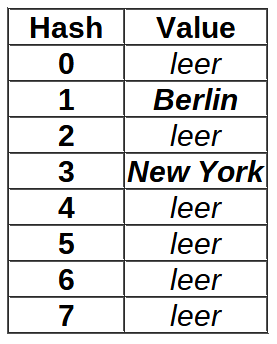
\includegraphics[scale=0.5]{Bilder/Hashmap_example_basic.PNG}
    \caption[Bild 1:]{Beispiel einer einfachen Hashmap}
     
\end{figure}

Versucht man jetzt aber beispielsweise die Stadt \textit{Paris} mit dem Key $K = 9$ einzufügen, so würde man mit der gewählten Hashfunktion den Eintrag ebenfalls an der Stelle 1
vornehmen, da $9~ mod~ 8 = 1$ gilt. Somit ist es zu einer Kollision gekommen. Wie damit umzugehen ist, hängt von der Implementierung ab, jedoch ist klar, das man das 
Auftreten solcher Kollsionen vermeiden möchte. Hierfür muss man eine geeignete Hashfunktion auswählen.
\subsection{Verschiedene Typen von Hashmaps}
\subsubsection{Offene Hashmaps}
Im vorherigen Abschnitt wurde das Problem der Kollision von Hashwerten bei der Verwendung von Hashfunktionen angesprochen.
Neben der Möglichkeit eine Funktion zu implementieren, welche sehr wenige solcher doppelter Hashes ausgibt, gibt es auch alternative Herangehensweisen.
Eine davon ist das Konzept der offenen Hashmap. Hierbei handelt es sich um eine Abwandlung des ursprünglichen Bauplans einer Hashmap.\\
Die klassische Funktionsweise sieht bei einer Kollision von Hashes keine genaue Handlungsweise vor. Man könnte den ursprünglich in einem Eintrag 
gespeicherten Wert durch den neuen überschreiben oder aber man nutzt den Ansatz der offenen Hashmap.
Bei diesem überschreibt man die alten Daten nicht durch die neuen, sondern man speichert die Daten, deren Hash mit dem eines bereits vorhandenden Datensatzes 
kollidiert, an die nächste freie Position in der Hashmap.
Für dieses Vorgehen sind zwei zusätzliche Funktionalitäten notwendig.\\
Erstens muss eine Suche über die gesamte Hashmap implementiert werden, bei der alle Listenelemente darauf geprüft werden, ob sie bereits belegt sind oder nicht.
Um dies zu entscheiden, muss dem Listenelement eine weitere Eigenschaft hinzugefügt werden. Es umfasst nicht mehr nur den die Daten, sondern auch den Key, denn ohne
ihn wären die Daten nun nichtmehr eindeutig zu identifizieren.
Die Suche nach einem Datensatz mittels seines Schlüssels würde ohne die Hinzunahme des Schlüssels selbst zum entsprechenden Datensatz, immer nur das erste Element der Liste 
ausgeben, welches durch Eingabe des Keys in die Hashfunktion den kollidierenden Hash ergab. Da eine Hashfunktion, wie bereits erwähnt, nicht umkehrbar ist, ist es notwendig,
den Schlüssel mitzuspeichern. So kann man nach Ermittelung des Hashes noch durch die Überprüfung durch den Key feststellen, ob es sich um den tatsächlich gesuchten Datensatz handelt.\\\\
Betrachtet man das Beispiel aus Abschnitt 2.2, dann würde die Hashmap nach dem Einfügen der drei Datensätze folgendermaßen aussehen:\\


\begin{figure}[h]
    \centering
    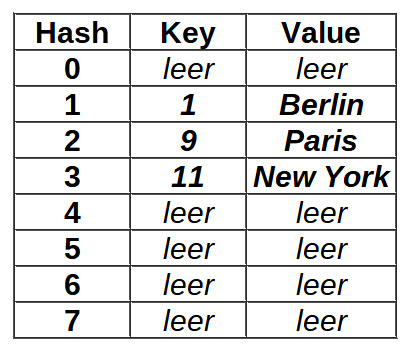
\includegraphics[scale=0.5]{Bilder/Hashmap_example_open.PNG}
    \caption[Bild 1:]{Beispiel einer offenen Hashmap}
     
\end{figure}
Der Datensatz \textit{Paris} mit dem Key \textit{K = 9} wird also an der Stelle 2 gespeichert, da Stelle 1 bereits belegt war.
Auserdem wurden zu allen Datensätzen auch die Keys gespeichert, damit bei der Suche nach einem Datensatz die Eindeutigkeit gewährleistet bleibt.\\
Der Nachteil dieser Implementierung ist, dass sie bei vielen Kollisionen das Problem hervorruft, dass die schnelle Suche, welche eine der wesentlichen Eigenschaften der Hashmap ist, leidet.
Dadurch, dass Speicherplätze mit Daten belegt sind, welche garnicht den eigentlichen Hash dieses Platzes besitzen, muss die Suche nach dem eigentlichen Datensatz dann wieder umständlicher durchgeführt werden.
Beispielsweise würden dann alle Speicherzellen um den eigentlichen Speicherort nach dem richtigen Datensatz überprüft werden, was eindeutig langsamer ist als die normale Hashmapsuche.
Durch geschickte Suchalgorithmen kann man die Effektivität dieser Suche zwar wieder steigern, aber sie ist doch nicht optimal.
Im schlimmsten Fall beträgt die Suchkomplexität allerdings $O(n)$ wobei $n$ die Anzahl der Elemente der Hashmap bezeichnet.

\subsubsection{Linked Hashmaps}
Eine andere Herangehensweisen im Vergleich zur \textit{offenen Hashmap} stellt die \textit{Linked Hashmap} dar. Wie der Name bereits andeutet, wir hier nicht nur ein Datensatz pro Hashmapelement gespeichert, 
sondern eine verkettete Liste (LinkedList). Diese Liste stellt eine Schachtelung der Elemente der Hashmap dar. Jedes Element umfasst dabei eine eigene LinkedList, welche wiederum drei Eigenschaften pro
Listenelement aufweist. Diese sind der Schhlüssel der Daten, die Daten selbst und ein Pointer auf den nächsten Eintrag der LinkedList.
Dieser Poniter ist der essenzielle Unterschied zum Ansatz der offenen Hashmap.\\
Anstatt bei einer Kollision den zweiten - den kollidierenden - Eintrag in ein neues Element der Hashmap zu speicher, wird hier das Hashmapelement benutzt, welches auch wirklich den gleichen Hash besitzt, 
wie er aus der Hashfunktion hervorgeht. Die Einträge werden also nacheinander in der Reihenfolge ihres auftretens in eine verkettete Liste gespeichert, deren Elemente vom ersten bis zum letzten um je einen 
Pointer auf den jeweiligen Nachvolger verbunden sind.
Die Suche kann dann für den jeweils durch Eingabe des Keys in die Hashfunktion ermittelten Hashwert für die dadurch eindeutig bestimmte LinkedList durchgeführt werden.
Ist das erste Element der Liste nicht das, dessen Key mit dem eingegebenen übereinstimmt, wird das nächste Element der Liste überprüft, welches durch den Poniter des Vorgängers refferenziert wird und so weiter bist
der gewünschte Eintrag an Daten gefunden wurde.
Am Beispiel aus Abschnitt 2.2 sähe das dann so aus:
\pagebreak

\begin{figure}[h]
    \centering
    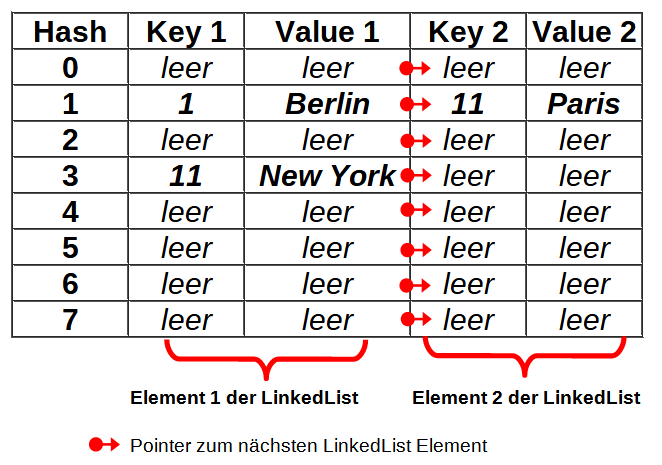
\includegraphics[scale=0.5]{Bilder/Hashmap_example_linked.PNG}
    \caption[Bild 1:]{Beispiel einer Linked Hashmap}
     
\end{figure}
Der Nachteil dieses Konzeptes ist, dass auch eine LinkedList nicht unbegrenzt lang sein kann, und selbst wenn sie es könnte hätte die Suche nach dem richtigen Listenelement 
im schlimmsten Fall eine Suchkomplexität von $O(n)$ wobei $n$ die Anzahl der Listenelemente ist.\\

\section{Implementierung}
\subsection{Package}
Da die Umsetzung und Implementierung einer Hashmap in C als Bibliothek umzusetzen sein sollte, umfasst diese zwei Dateien.
Das Headerfile, \lstinline{hashmap.h}, welches alle Definitionen und Deklarationen für neue Datentypen und und Funktionen umfasst, die 
\lstinline{hahsmap.c} Datei, welches die Initialisierung aller Hashmap-Funktionen und alle Funktionalitäten umfasst.\\
Zusätzlicg existiert im Package ein Makefile, welche für die Compilierung der Files und das Linken der Bibliotheken sowie Objektdateien 
verantwortlich ist.\\
Im wesentlichen lässt sich die Implementierung in folgendem UML-Diagramm gut darstellen. Es weißt zwei Klassen aus, die Klasse der \lstinline{Hashmap}, 
und die des \lstinline{Hashmap_Elements}. Letzteres bezeichnet die Daten, welche in der Hashmap gespeichert werden sollen.\\
Da es in der Programmiersprach C allerdings keine Klassen gibt, wird statt dessen zwei Structs verwendet, welche die Eigenschaften der 
\lstinline{Hashmap} und des \lstinline{Hashmap_Elements} umfassen soll. Alle Funktionen, welche zum erstellen, einfügen, löschen von Datensätzen und der Hashmap selbst dienen, werden 
mit Pointern auf diese Structs arbeiten.\\

\begin{figure}[t]
    \centering
    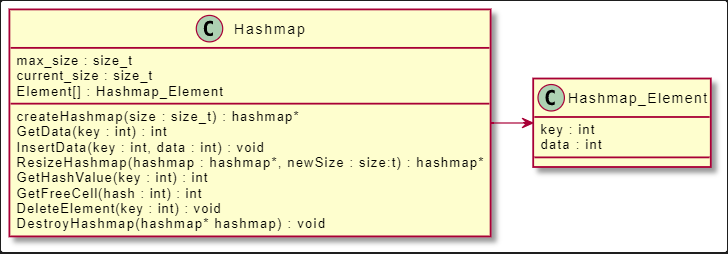
\includegraphics[scale=0.5]{Bilder/UML.PNG}
    \caption[Bild 1:]{UML-Diagramm der angedachten Implementierung.}
     
\end{figure}

Bei der Umsetzung der Hashmap-Implementierung wurde ausschließlich das Konzept der offenen Hashmap umgesetzt, auch die Hashfunktion wurde sehr simpel gehalten.
Es handelt sich um die bereits erläuterte Modluo-Operation.\\
Auch wenn die Nachteile bereits angeführt wurden, soll in dieser Arbeit nur die grundsätzliche Funktionalität 
einer Hashmap umgesetzt werden und dafür reicht diese Hashfunktion völlig aus.\\


\subsection{Hashmap Struct}
Das Kernstück der Implementierung bildet der Datentyp der Hashmap, genauer das Struct, welches als Hashmap fungieren soll.\\
Dieser Umfasst im Wesentlichen drei Eigenschaften. Die maximale Größe der Hashmap \lstinline{max_size}, welche als nicht-negative 
ganze Zahl, als \lstinline{size_t} gespeichert wird und die aktuelle Größe der Hashmap, das heißt die aktuelle Anzahl an gespeicherten 
Elementen, \lstinline{current_size} - ebenfalls ein \lstinline{size_t}. Die dritte Komponente des Structs \lstinline{hashmap} ist das 
\lstinline{hash_element}, welches ein Pointer auf ein Array aus \lstinline{hashElement} Structs darstellt. In dieses Array werden die Daten 
gespeichert, welche in die Hashmap eingefügt werden sollen.\\

\begin{lstlisting}[language=C]
    typedef struct hashmap{

        size_t max_size;
        size_t current_size;
        hashElement* hash_element;
        
    } hashmap;
\end{lstlisting}

Das \lstinline{hashElement} Struct selbst besitzt ebenfalls drei Variablen. Da es sich bei dieser Implementierung um eine reine Integer 
Umsetzung des Hashmap-Konzepts handelt, sind sowohl die \lstinline{key} als auch die \lstinline{data} Variable vom Datentyp \lstinline{int}.
Wie die Namen schon andeuten werden in \lstinline{key} die Schlüsselwerte und in \lstinline{data} die Daten gespeichert. Für die Markierung ob 
ein Eintrag bereits genutzt wurde oder nicht, wird das Feld \lstinline{entryUsed} verwendet. Dabei handelt es sich um einen selbst definierten 
Datentyp \lstinline{HASHMAP_BOOL}.\\

\begin{lstlisting}[language=C]
    typedef struct hashElement {

        int key;
        int data;
        HASHMAP_BOOL entryUsed;

    } hashElement;
\end{lstlisting}

Der \lstinline{HASHMAP_BOOL} Datentyp soll die in der Programmiersprache C nicht vorhanden bool'schen Datentypen emulieren. Es handelt sich dabei
schlicht um zwei Typendefinitionen der Intergerwerte $0$ und $1$. In C werden \textit{false} als $0$ und \textit{true} als $\neq 0$ interpretiert.
Um nicht auf den Wert einer Variablen achten zu müssen, wurden die \lstinline{HASHMAP_BOOL} Datentypen folgendermaßen definiert:\\

\begin{lstlisting}[language=C]
    typedef int HASHMAP_BOOL;
    #define HASHMAP_BOOL_TRUE    1
    #define HASHMAP_BOOL_FALSE   0
\end{lstlisting}


\subsection{Hashmap erstellen}
Bevor man Daten in eine Hashmap speichern kann, muss man diese natürlich zuvor erstellen. Hierzu initialisiert man den Hashmap Datentypen 
erst einmal auf dem \textit{Stack}. Der \textit{Stack} stellt einen Teil des Speichers eines Systems dar. Hier werden Daten wie auf einem 
Namensgebenden Stapel gespeichert. Man muss sich den Speicher nicht vorher reservieren, da im vorhinein bekannt ist, wie groß der benötigte 
Speicherbereich ist, den man benötigt. Das spart Resourcen und Zeit. Diese Initialisierung sähe wie folgt aus:\\

\begin{lstlisting}[language=C]
    hashmap map;
    initHashmap(&map , 8);
\end{lstlisting}

Die Funktion \lstinline{initHashmap()} bekommt als Eingabewerte einen Pointer auf die zuinitialisierende Hashmap, in diesem Fall \lstinline{&map} 
und eine maximale Größe, welche die Hashmap nach der Initialisierung haben soll. Diese Größe beträgt hier 8 Elemente.\\
Die Funktionsweise der Initialisierungsfunktion  \lstinline{initHashmap()} sieht nun wie folgt aus:\\

\begin{lstlisting}[language=C]
    int initHashmap(hashmap* hm, size_t size)
    {   int error;
    
        hashElement* hm_elements;

        hm_elements = (hashElement*) malloc(size * sizeof(hashElement));
        if(!hm_elements){
                error = HASHMAP_CREATE_ERROR;
        } else error = HASHMAP_SUCCESS;

        hm->current_size = 0;
        hm->max_size = size;
        hm->hash_element = hm_elements;

        return error;
    }

\end{lstlisting}

Zuerst werden eine Variablen declariert. Es handelt sich um die \lstinline{int error} Variable, welche für die Fehlerbehandlung als 
Zwischenspeicher für den Fehlercode dient. Im Abschnitt über die Fehlerbehandlung (3.8) wird hierauf näher eingegangen.\\
Es folgt die Initialisierung des Arrays für die Hashmapelemente. Dieser wird über die Funktion \lstinline{malloc()} bewerkstelligt.
Somit liegt dieses Array auf dem Heap, einem Speicherbereich, auf dem man die Größe des Speichers zuvor reservieren muss. Man kann die Größe 
dann aber auch zur Laufzeit des Programms ändern. Das wird im Abschnitt 3.7 eine größere Rolle spielen, denn dort geht es um die automatische 
Veränderung der Größe der Hashmap.\\
Zuletzt werden noch alle Felder der Hashmap initialisiert und zugewiesen und der Fehlercode ausgegeben.

\subsection{Hashmap löschen}

    Das Löschen der Hashmap ist wichtig und muss daher gesondert betrachtet werden.\\
    Da das Array \lstinline{hm_elements} auf dem Heap mittels \lstinline{malloc()} initialisiert wurde, muss dieser reservierte Speicherbereich 
    auch wieder freigegeben werden. Anderenfalls würde über kurz oder lang dieser Speicher völlig überfüllt sein mit ungenutzten Datenfragmenten.
    Hierfür dient die Funktion \lstinline{destroyHashmap()}. Alles, was diese Funktion bewerkstelligt, ist, dass sie das \lstinline{hm_elements} 
    Array einer gegebenen Hashmap frei gibt.\\

\begin{lstlisting}[language=C]

    void destroyHashmap(hashmap* hm)
    {   
        free(hm->hash_element);
    }
\end{lstlisting}
\pagebreak

\subsection{Daten einfügen, lesen und löschen}

Nachdem die Hashmap jetzt erstellt und auch sauber wieder gelöscht werden kann, ist der nächste Schritt das Einfügen der Daten.
Hierzu dient die Funktion \lstinline{insertData()}. Ihre Eingabewerte sind \lstinline{int key}, \lstinline{int data} und der Pointer auf die Hashmap 
\lstinline{hashmap* hm}.\\
Zuerst wird in dieser Funktion überprüft, ob die aktuelle Größe der Hashmap bereits den Maximalwert erreicht hat. Wenn dem so ist, dann wird die Funktion 
\lstinline{resizeHashmap()} aufgerufen, um die Hashmap zu vergrößern, aber dazu mehr in Abschnitt 3.7.\\
Danach wird der Hashwert mittels der Hashfunktion durch den Aufruf \\
\lstinline{getHashValue(key, hm->max_size)} ermittelt. Im Abschnitt 3.6 wird nocheinmal darauf eingegangen.\\
Ist das geschehen muss, nach dem Ansatz der offenen Hashmap, überprüft werden, ob der Eintrag in den \lstinline{hm_elements}, der dem Hashwert entspricht, 
noch frei ist. Sollte dem nicht so sein, dann wird die Hashmap nach dem nächsten freien Eintrag abgesucht und die Daten stattdessen dort eingefügt. 
All das wird durch eine Überprüfung mittels \lstinline{if ()} und einer \lstinline{for}-Schleife durchgeführt.\\

\begin{lstlisting}[language=C]

if (hm->hash_element[hash].entryUsed == HASHMAP_BOOL_TRUE || (size_t)hash > hm->max_size){

    //hash collision happened

    int newHash = 0;
    for (size_t i = 0; i < hm->max_size; i++){
        if (hm->hash_element[i].entryUsed == 
            HASHMAP_BOOL_FALSE) newHash = i;
    }

    hm->hash_element[newHash].key = key;
    hm->hash_element[newHash].data = data;
    hm->hash_element[newHash].entryUsed = HASHMAP_BOOL_TRUE;
    hm->current_size++;

} else {

    //no collision
    hm->hash_element[hash].key = key;
    hm->hash_element[hash].data = data;
    hm->hash_element[hash].entryUsed = HASHMAP_BOOL_TRUE;
    hm->current_size++;

}

\end{lstlisting}

Das Lesen der Daten wird auf ganz ähnliche Weise in der Funktion \lstinline{getData()} durchgeführt.
Zuerst wird auf einem gegeben Key ein Hashwert mittels der Funktion \lstinline{getHashValue(key)} ermittelt. Danach wird überprüft, ob der Eintrag an der Stelle \lstinline{hm->hm_elements[hash]} auch 
den richtigen Key besitzt wie der gesuchte Datensatz. Ist das der Fall, dann werden die Daten ausgegeben, ansonsten wird die Hashmap 
abgesucht ob der gewünschte Datensatz an einer anderen Stelle des Arrays liegt.\\

Auf gleiche Art wird das Löschen eines Datensatzes in der Funktion \lstinline{deleteData()} umgesetzt. Die Suche wird nach dem gleichen Prinzip durchge-
führt, nur dass die Daten nicht ausgegeben, sondern gelöscht werden, indem die Werte für \lstinline{hm->hm_elements[hash].key} und \lstinline{hm->hm_elements[hash].data} 
auf $~0$ gesetzt werden und dem Eintrag \lstinline{hm->hm_elements[hash].entryUsed}, welcher beim Einfügen auf \lstinline{HASHMAP_BOOL_TRUE} gesetzt wurde, jetzt der Wert \lstinline{HASHMAP_BOOL_FALSE} zugewiesen wird.\\
Zusätzlich wird an dieser Stelle dann überprüft, ob die aktuelle Größe der Hashmap $1/4$ der maximalen Größe unterschhreitet. Wenn dem so ist, wird die Hashmap auf dieses Viertel gesetzt. Das 
geschieht mittels der Funktion \lstinline{resizeHashmap()}. Mehr dazu im Abschnitt 3.7.

\subsection{Einfache Hashfunktion}

Bei allen Einfüge-, Lese- oder Löschungsoperationen für Datensätze der Hashmap spielt die Hashfunktion in Form von \lstinline{getHashValue()} eine wichtige Rolle.
Wie bereits beschrieben handelt es sich bei dieser Funktion um die Modulo-Operation, auch wenn diese aus bereits beschriebenen Gründen für die Praxis nicht geeignet ist.
Der Einfachheit halber wurde sie dennoch verwendet, allerdings mit einer minimalen Abweichung zur rein mathematischen Version dieser Operation.\\
Da der Key vom Typ \lstinline{int} ist, kann dieser auch negativ sein. Bei der Modulo-Operation würde dies allerdings für einen negativen Rückgabewert bewirken.
Mathematisch ist das völlig korrekt aber es verursacht ein Problem in der Implementierung der Hashmap. Da der Hashwert als Index für das Array \lstinline{hm_elements} benutzt wird, 
käme ein negativer Index hier eine Verletztung der Schreib- und Lesezugriffsrechte gleich. Um das zu verhindern, wird vom Ergebnis der Operation noch der Absolutbetrag gebildet. 
Dadurch entstehen zwar einige zusätzliche Kollisionen aber das spielt bei der ohnehin kollisionsreichen Modulo-Operation keine größere Rolle mehr.\\
Folglich sieht die Implementierung dann folgendermaßen aus:\\

\begin{lstlisting}[language=C]
    int getHashValue(int key, size_t hm_size)
{   
    int hash = key % hm_size;

    return abs(hash);
}
\end{lstlisting}


\subsection{Automatische Größenanpassung der Hashmap}

In einigen Fällen ist es von Vorteil, dass die Hashmap ihre Größe automatisch ändert. Möglicherweise kann man vorher nicht abschätzen, wie viele Elemente 
man in diese Datenstruktur einfügen möchte. In anderen Fällen kann es auch nützlich sein. Hat man eine große Menge an Datensätzen gelöscht, dann nimmt die 
Hashmap dennoch den gleichen Platz wie zuvor ein, da dieser zuvor reserviert wurde. Um diesen Speicherbereich nicht unnötig zu blockieren, existiert die Funktion 
\lstinline{resizeHashmap()}. Sie bekommt einen Poniter auf eine Hashmap \lstinline{hashmap* hm} und eine neue maximale Größe \lstinline{size_t size} als Eingabewerte.\\
Zuerst müssen zwei Pufferarray reserviert werden, indem alle in der Hashmap befindlichen Daten zwischengespeichert werden können. Eines für die Schlüssel und eins für die Daten.
Jetzt kann das Array \lstinline{hm_elements} mittels der Funktion \lstinline{realloc()} auf seine neue Größe gesetzt werden.
Danach können die Datensätze dann wieder mittels der Funktion \lstinline{insertData()} in die Hashmap eingefügt werden. Da die Hashwerte von der Größe der Hashmap abhängen, 
werden die Hashwerte neu berechnet anstatt diese zuvor zu speichern.\\
Zuletzt werden die Puffer wieder freigegeben, denn diese wurden zuvor mittlets \lstinline{malloc()} reserviert. Das geschieht wieder durch den Aufruf der Funktion \lstinline{free()}.

\subsection{Fehlerbehandlung}

Die Fehlerbehandlung hat eine eigene Funktion. Alle Funktion geben jeweils einen Fehlercode aus, welche in der Variable \lstinline{int error} dieser Funktion gespeichert wird.
Die Fehlercodes wurden in der Headerdatei \lstinline{hashmap.h} festgelegt.\\

\begin{lstlisting}[language=C]
    
    #define HASHMAP_SUCCESS         0  
    #define HASHMAP_OVERLOAD        1  
    #define HASHMAP_INPUT_ERROR     2  
    #define HASHMAP_OUTPUT_ERROR    3  
    #define HASHMAP_CREATE_ERROR    4  
    #define HASHMAP_RESIZE_ERROR    5 

\end{lstlisting}

Die Fehlerausgaben werden in der Funktion \lstinline{errorHandling()} umgesetzt. Sie besteht aus einem \lstinline{switch}-Statement, welches zwischen den 
Fehlercodes unterscheidet.

\begin{lstlisting}[language=C]
    
    void errorHandling(int error)
{
        switch (error)
        {
            case HASHMAP_SUCCESS: 
                printf("No errors occured!\n");
                break;
            case HASHMAP_OVERLOAD:
                printf("Error! Hashmap is full!\n"); 
                break;     
            case HASHMAP_INPUT_ERROR:  
                printf("Error! Could not insert element.\n"); 
                break;
            case HASHMAP_OUTPUT_ERROR: 
                printf("Error! Could not find or extract 
                element.\n");
                break;
            case HASHMAP_CREATE_ERROR:
                printf("Error! Could not create hashmap.\n");
                break;
            case HASHMAP_RESIZE_ERROR: 
                printf("Error! Could not resize hashmap.\n");
                break;
        }
    }

\end{lstlisting}

\section{Benchmarking}

Was die Leistungsfähigkeit dieser Implementierung angeht, ist von vorherein klar, dass sie nicht optimal sein kann. Vorallem die Hashfunktion 
Zieht die Geschwindigkeit, mit der die Suche und das Einfügen eines Datensatzes gescheiht, sehr nach unten. Fügt man allerdings nicht hunderttausende 
Werte ein, so ist diese schmälerung nahezu vernachlässigbar. Exemplarisch werden im folgenden drei der Zeit, welche beim Einfügen der Datensätze auftritt, die Zeit zum Einfügen eines Datensatzes, die Dauer der Einfügeoperation aller Datensätze und die durchschnittliche 
Lesedauer für ein Element aufgeführt. Dabei wird jeder Test 2000 mal durchgeführt, einmal mit 100, einmal 1000 und einmal mit 10000 Elementen, welche zufällig generiert werden.
Dabei liegt die Obergrenze für den Schlüsselwert bei 10000 und die Untergrenze bei -100, die Wahl dieser Grenzen ist willkürlich.\\
\begin{figure}[h]
    \centering
    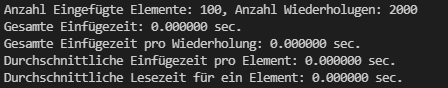
\includegraphics[scale=0.5]{Bilder/100e.PNG}
    \caption[Bild 5:]{Benchmarking mit 100 x 2000 Elementen}

\end{figure}
\begin{figure}[h]
    \centering

    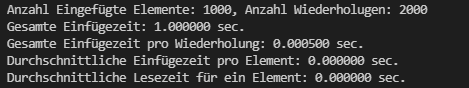
\includegraphics[scale=0.5]{Bilder/1000e.PNG}
    \caption[Bild 6:]{Benchmarking mit 1000 x 2000 Elementen}

\end{figure}
\begin{figure}[h]
    \centering
    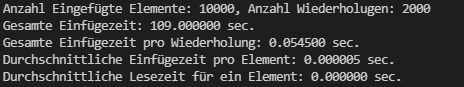
\includegraphics[scale=0.5]{Bilder/10000e.PNG}
    \caption[Bild 7:]{Benchmarking mit 10000 x 2000 Elementen}
\end{figure}
\linebreak
Es wird ersichtlich, dass die Einfügezeit sehr schnell mit der Anzahl der eingefügten Elemente wächst. Die Suchzeit hingegen bleibt sehr klein, trotz der ungünstig gewählten Hashfunktion.
Dafür sind die Keys verantwirtlich, welche bei wenigen Elementen eine hohe Wahrscheinlichkeit haben, eindeutig zu sein, da die Spanne für die Zufallszahl sehr groß ist.\\
Um noch einen Vergleich zwischen verschiedenen Hashfunktionen anzubringen, folgt eine Grafik mit wesentlich komplexeren Funktionen, welche teilweise noch in der Praxis für 
kryptografische Zwecke verwendet werden. Bei diesen ist es besonders wichtig wenige Kollisionen zu verursachen. Dennoch liegt ihre Ausführungszeit im Mykrosekundenbereich, was sehr schnell ist.\\
\begin{figure}[h]
    \centering
    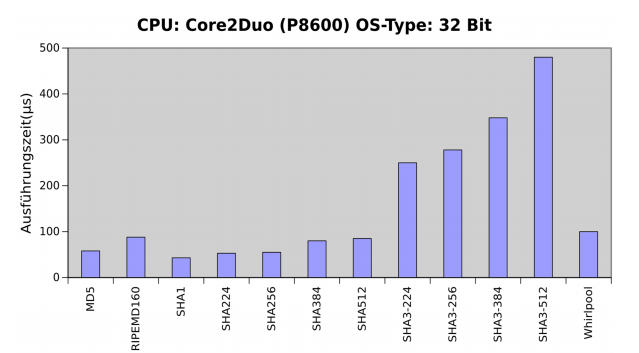
\includegraphics[scale=0.5]{Bilder/hashfunctions_diag.png}
    \caption[Bild 8:]{Verschiedene Hasfunktionen im Vergleich}
\end{figure}


\section{Zusammenfassung}
Zusammenfassend gibt es einige Dinge zu sagen. 
Zu allererst ist anzumerken, dass die verwendete Hashfunktion, die Modulo-Operation,
bereits eingangs als eigentlich ungeeignet beschrieben wurde. Für den rein akademischen Fall, worum es sich bei dieser Arbeit jedoch 
handelt, reicht sie aus, um die grundsätzliche Funktionalität einer Hashmap umzusetzen.\\
Auch gibt es einige zusätzliche Funktionen, die ich allerdings nicht umgesetzt habe, weil die Zeit zu knapp war.
Hier wäre zum Beispiel die Auswahl zwischen verschiedenen Hashfunktionen und das Festlegen der Grenze für die Resize-Funktion zu nennen.
Beides sind sogenannte "comfort of life" Änderungen und damit nicht zwingend für die Umsetzung erforderlich.
In diese Kategorie gehört auch eine Mögliche Implementierung der Auswahl zwischen dem Ansatz der offenen Hashmap und dem der Linked Hashmap.\\\\
Ansonsten ist das Konzept der Hashmap umgesetzt worden, jedoch nicht so optimal, wie es bei einer professionellen Umsetzung der Fall wäre.
Hier wäre eine effektiere Nutzung des Speichers und effizientere Programmierung der Funktionen der Hashmap denkbar.\\
Die letzte noch angedachte Änderung wäre die Erweiterung der Bibliothek von ausschließlich Integer Datentypen auf 
mehere mögliche Datentypen mittels Pseudogenerics.\\
Abseits dessen funktioniert die Hashmapbibliothek ohne Probleme und könnte, unter der Maßgabe der Nutzung von ausschließlich Intergern, genutzt werden.

\section{Quellen}
\begin{itemize}
\item[[1]] $https://de.wikipedia.org/wiki/Assoziativspeicher$
\item[[2]] $https://www.ionos.de/digitalguide/server/sicherheit/hashfunktion/$
\item[[3]] $https://de.wikipedia.org/wiki/Hashfunktion$
\item[[4]] $http://www.codeadventurer.de/?p=2091$
\item[[5]] $https://www.syssec.at/de/veranstaltungen/dachsecurity2017/ \\
            ~~~~~~~~papers/DACH_Security_2017_Paper_13B2.pdf$
\end{itemize}
\centering 
Alle Quelle zuletzt besucht 01.10.2021

\pagebreak


\includegraphics[scale=1]{Bilder/sse.PNG}



\end{document}